%Following is an open list of problems that we will address in order to achieve device composition by means of implicit interaction.
%\begin{enumerate}
%\item{\emph{Setup}: How is a device enabled for integrating with a tabletop?
%The setup should be simple, to be performed only once by non-technical users.
%An initial survey of possible solutions points towards the use of tagging mechanisms and/or camera-based object recognition.}
%\item{\emph{Discovery}: How do the tabletop and the device discover and communicate with each other?
%How do we solve the issues of discovery, handshake, network connectivity, and encryption mechanisms to ensure privacy?}
%\item{\emph{UI transfer}: Given the computational constraints of mobile devices, how can the UI transfer be efficiently implemented so as to support native applications and guarantee a seamless user experience?}
%\item{\emph{Input}: How can the users interact with their applications on the tabletop (touch and other peripherals)?}
%\item{\emph{Interaction Design}: What means of interaction are best-fitted for the tabletop-based systems that we propose to develop?
%How can we best adapt to public/private uses and single/multiple users?
%How can we take advantage of the larger interaction surface?}
%\end{enumerate}

%%%%%%%%%%%%%%%%%%%%%%
%%% IMPLEMENTATION %%%
%%%%%%%%%%%%%%%%%%%%%%

\chapter{The TIDE prototype}
\label{system}

TIDE (Tabletop Interactive Display Extension) is a prototype that combines smartphones and tabletops by way of UI replication.
It was implemented in .NET for the Microsoft Surface (Windows Vista), referred to as MS in this chapter.
It was tested with an iPhone 4 running iOS 5 and a HTC Legend phone running Google Android 2.1, and it can be extended to support other smartphone models.

As shown in figure~\ref{fig:overview}, TIDE consists of three components, that are responsible for pairing, UI replication, and the surface UI.
Pairing is done through camera-based object detection.
TIDE relies on OpenCV (Open Source Computer Vision) \citep{opencv} to detect phone-like objects to connect to, and to track the devices during the application session.
The UI replication is based on the VNC protocol \citep{Richardson:1998:vnc}.
TIDE includes a VNC client that is based on the VncSharp library \citep{vncsharp}, and that connects over the network to a VNC server running on the smartphone (third-party application).

The surface UI is implemented using the Microsoft Surface SDK and WPF (Windows Presentation Foundations).
\\
\linebreak
Figure~\ref{fig:sequenceOverview} shows the basic interaction flow that TIDE supports.
First, the user places the smartphone the MS, which triggers the pairing process, described in section~\ref{sec:pairing}.
Section~\ref{sec:tracking} describes how smartphones are detected and tracked during TIDE application sessions.
Second, the smartphone's UI is replicated to the tabletop via the VNC protocol, as presented in section~\ref{sec:replicatedui}.
Lastly, the user interacts with the application via the surface UI, described in section~\ref{sec:surfaceui}.

\begin{figure}[t]
  \centering
    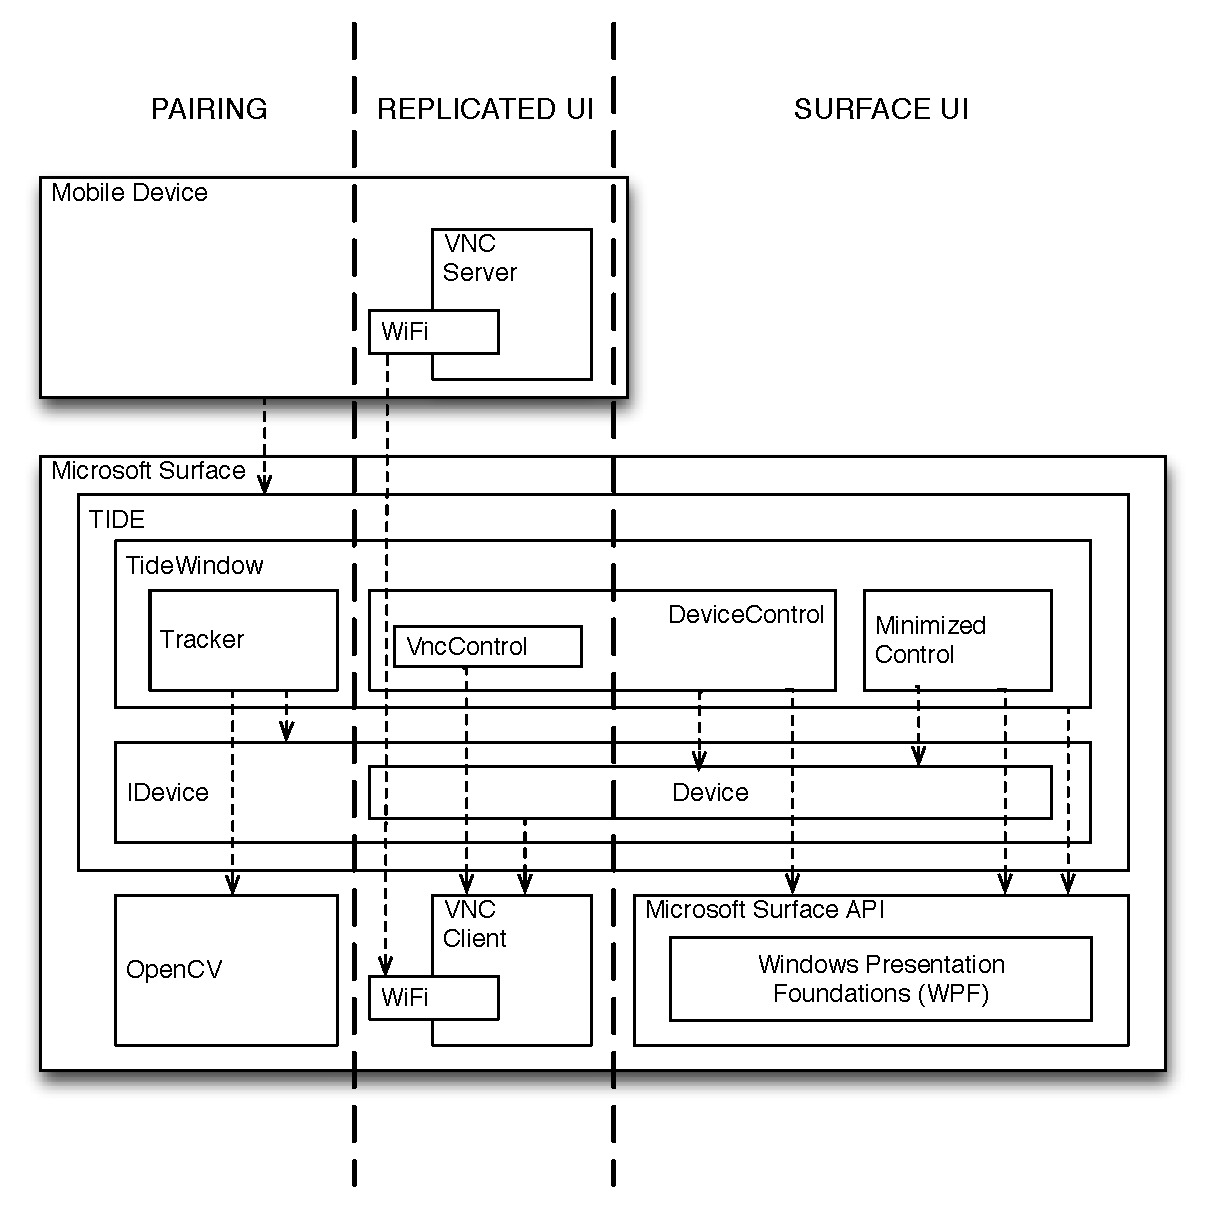
\includegraphics[width=0.8\textwidth]{images/overview}
    \caption{TIDE overview.}
    \label{fig:overview}
\end{figure}

\begin{figure}[h!]
  \centering
    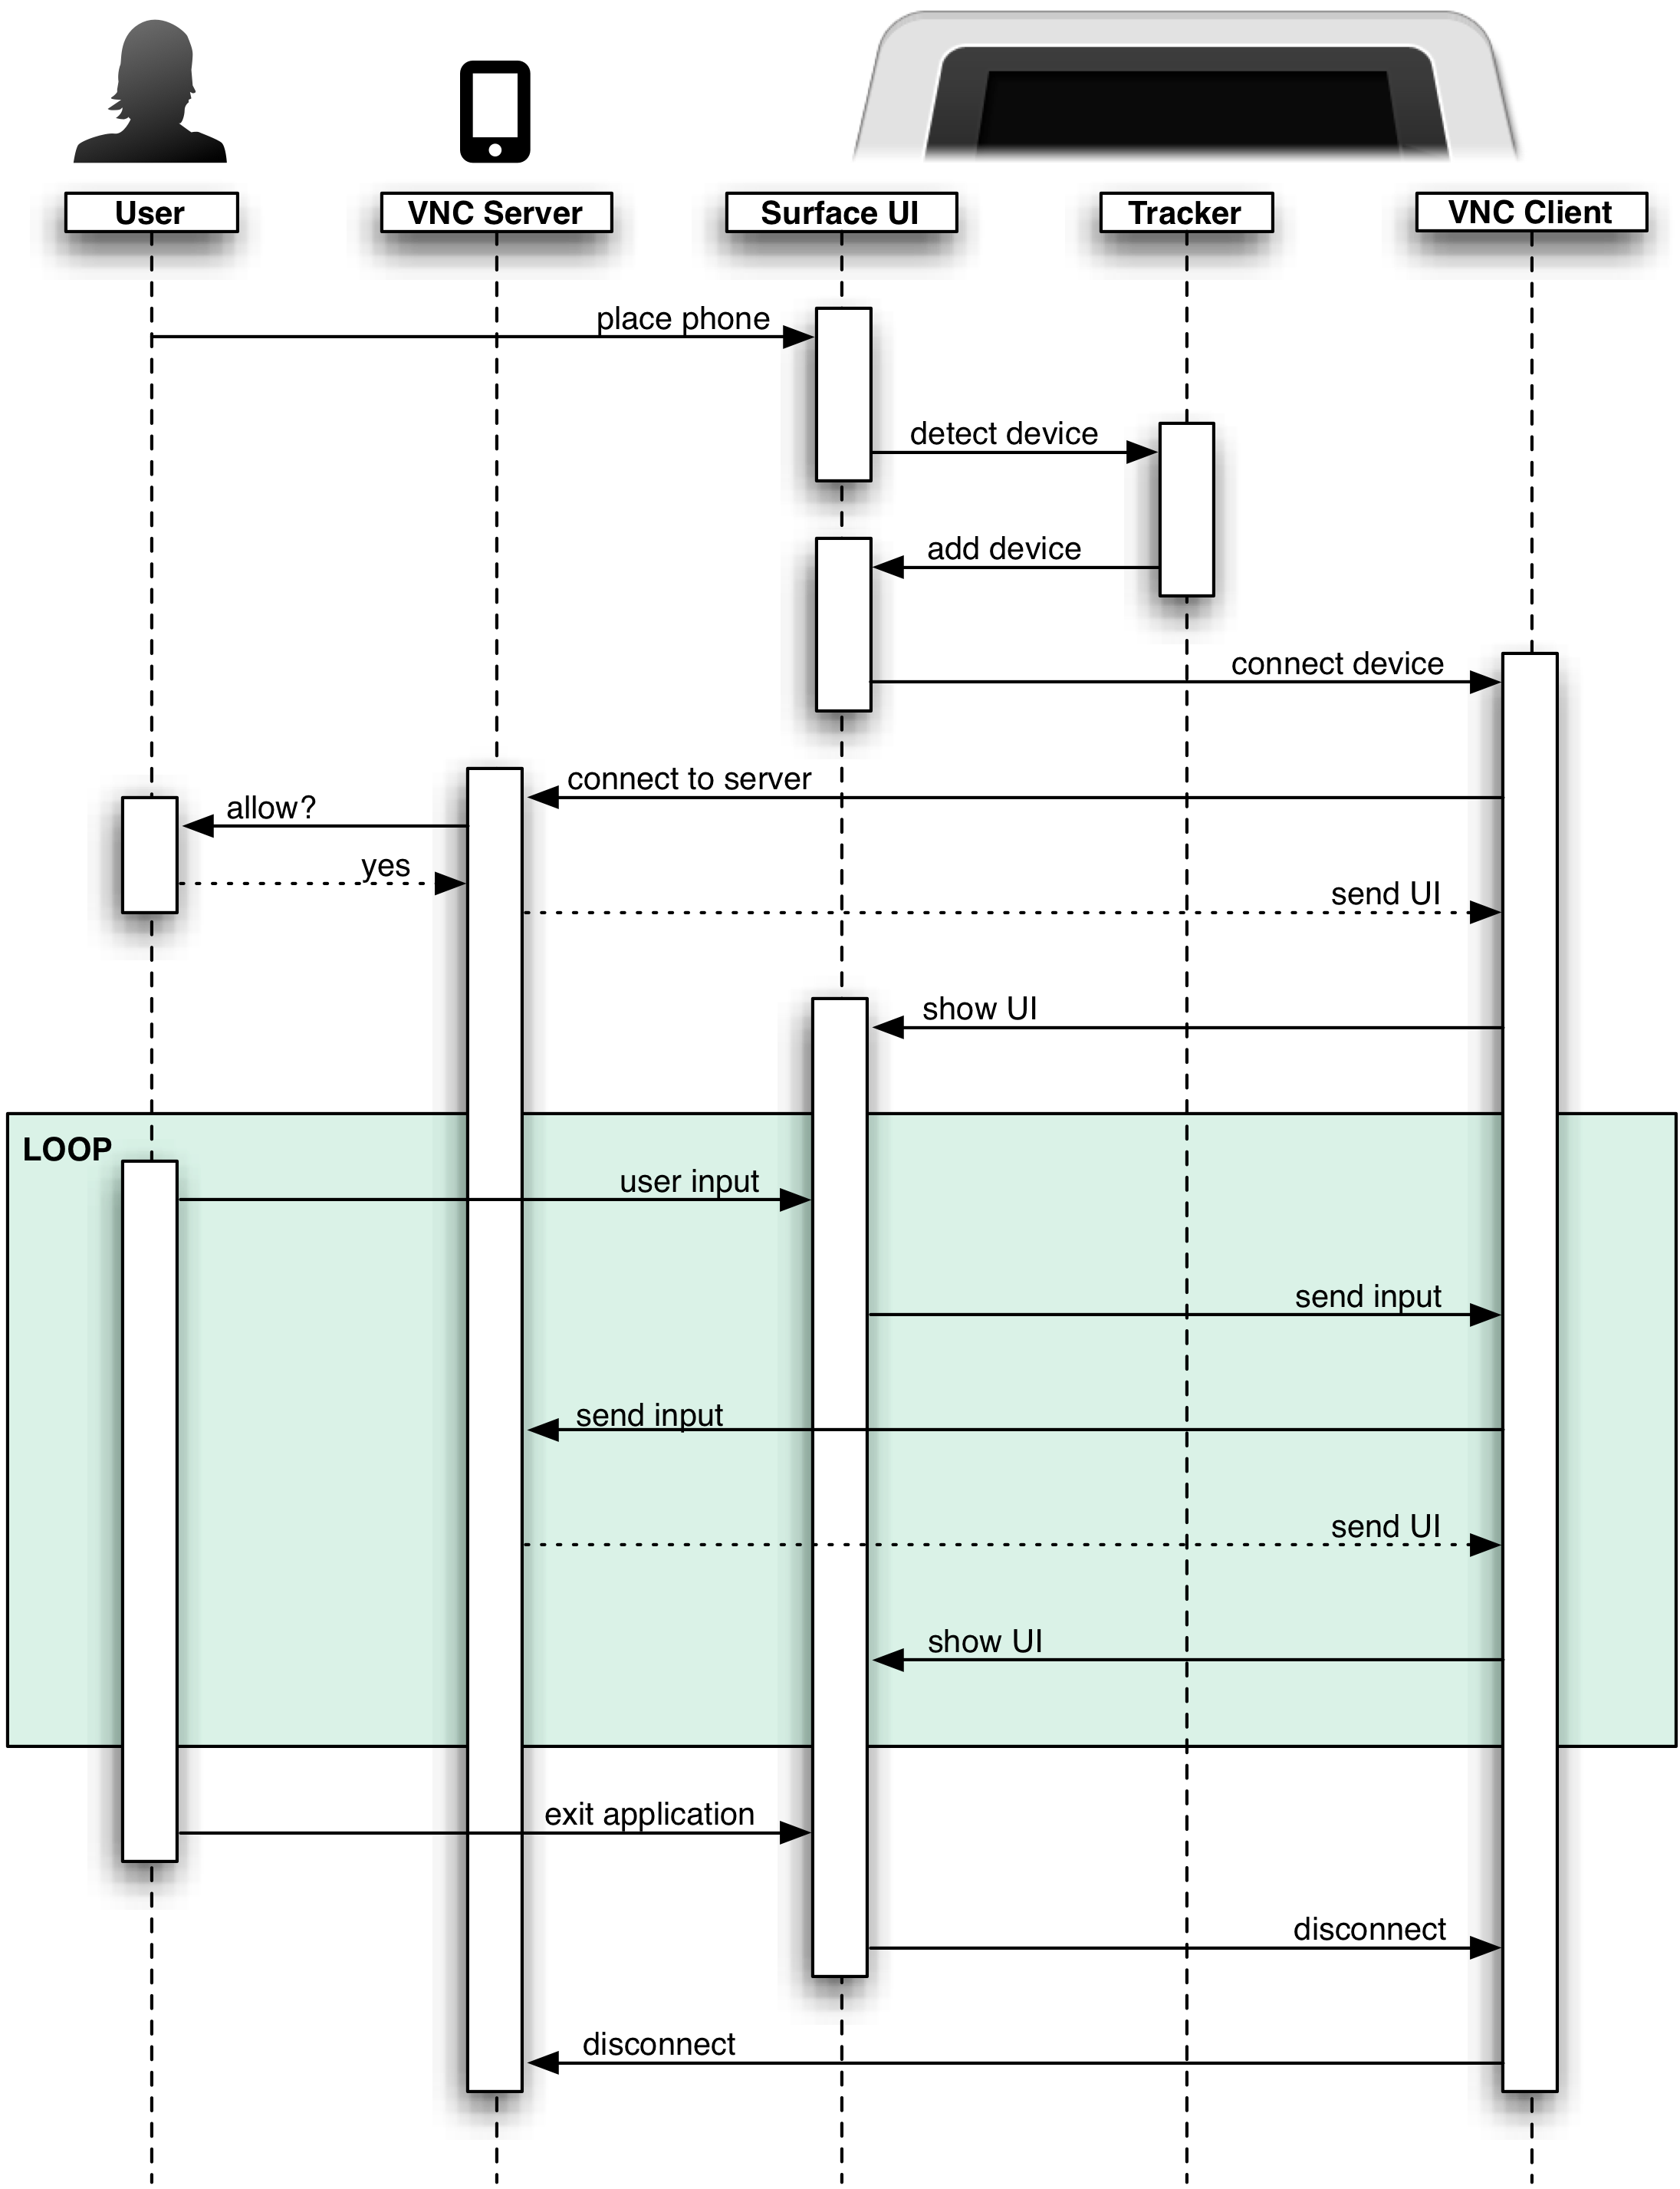
\includegraphics[width=0.8\textwidth]{images/sequenceOverview}
    \caption{TIDE overview.}
    \label{fig:sequenceOverview}
\end{figure}

%%%%%%%%%%%%%%
%% PAIRING %%
%%%%%%%%%%%%%%
\section{Pairing}
\label{sec:pairing}

The pairing procedure requires that both devices are connected to the local network.
In the case of the smartphone, this connection is very likely wireless.
Moreover, a VNC server instance should be up and running on the smartphone, for the system to function.

To achieve successful pairing, the following steps must be completed:
(1) a \emph{trigger} starts the procedure,
(2) \emph{discovery} allows the smartphone's local IP address to be made available to the tabletop and
(3) the \emph{connection} is established, given that the user explicitly authorizes it.

\subsection{Trigger}

To start the pairing procedure, a trigger must be used.
In TIDE, this trigger is provided by the detection of a smartphone object lying on the tabletop.

Interactive displays that are based on computer-vision technologies function by seeing the shape of the objects that come in contact with the surface.
That implies that not only are fingers seen, but also other objects such as books, cups, or cell phones.
The MS is an example of a tabletop that was designed for integrating with physical objects.
This strategy is based on the use of visual markers
[EXPLAIN MS VISUAL TAGS STRTATEGY HERE]

However, the MS camera-based system is able to see all contact shapes, as long as they reflect infra-red light.
The display's visual input can be captured and analyzed with computer vision algorithms such as the ones provided by OpenCV, and specific shapes can be recognized.
This strategy was used in the TIDE implementation, to detect specific smartphones, and trigger the procedure.
The details of the smartphone detection steps are explained in section~\ref{sec:tracking}.

The reason for using shape recognition instead of the MS tag recognition system is to remove as many constraints as possible, to make the system accessible to all, whatever the context.
Using visual tags would imply that the system be usable only by users that had applied a visual tag to the smartphone.

\subsection{Discovery}

The smartphone's local IP address must somehow be made available to the TIDE application, in order to establish the connection.

There is one easy solution to this problem, which is having the user enter the IP address in a dialog window on the tabletop, but this approach has serious limitations.
Finding out what the IP address is not obvious for most users, it requires digging into the networking settings of the phone.
In any case, it is a process of several steps.
Moreover, entering the address on the tabletop takes time and can lead to mistakes.
IP addresses are numeral strings of typically more then 10 digits, which makes them cumbersome to remember and type.

An easier solution is to automatize the discovery process, using networking protocols such as UPnP and Bonjour, based on Zeroconf.
[HOW MUCH SHOULD I EXPLAIN HERE??]
\\
\linebreak
Seeing that the focus of this work lies elsewhere, 
%is not to contribute within this area,
 and for reasons of time constraints, it was decided not to implement the discovery protocol.
The system currently functions with IP addresses hardcoded into the TIDE implementation on the MS, to serve the purpose of the present proof-of-concept.

\subsection{Connection}

To protect the user's privacy, the connection needs explicit authorization.
This is handled by a dialog that appears on the tabletop, described further in section~\ref{sec:surfaceui}.

The connection is otherwise handled by the VNC components on tabletop and smartphone, whose implementation details are presented in section~\ref{sec:replicatedui}.

%%%%%%%%%%%%%%
%% TRACKING %%
%%%%%%%%%%%%%%
\section{Tracking}
\label{sec:tracking}

\begin{figure}[htbp]
  \centering
    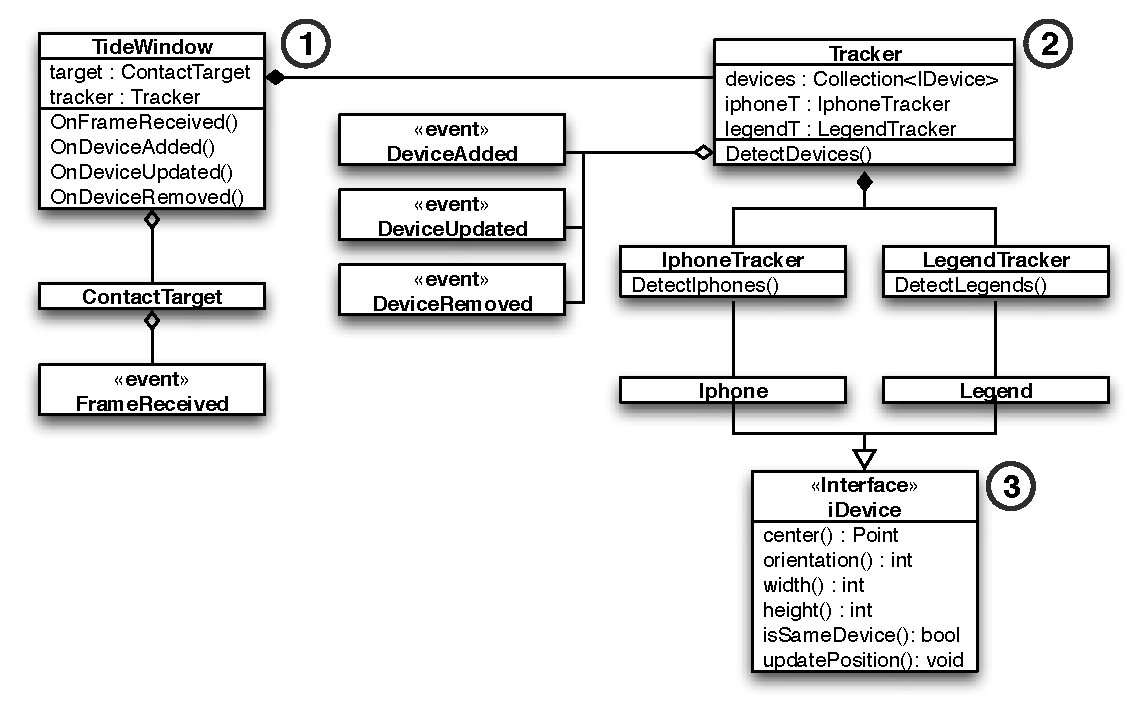
\includegraphics[width=1\textwidth]{images/trackingDiagram}
    \caption{Tracking overview.}
    \label{fig:trackingDiagram}
\end{figure}

The MS computer vision is based on infrared light that is projected towards the interactive display, and reflected by the objects that are in contact with it.
The reflection is captured by multiple cameras, and processed for system use.
By using OpenCV, it is possible to analyze the captured images to detect specific shapes and interpret the nature of the object on the table.

Figure~\ref{fig:trackingDiagram} shows the implementation of a mechanism that allows TIDE to detect specific smartphones, and track their whereabouts on the surface during application sessions.
The core layer of the Surface SDK provides the \texttt{ContactTarget} class, which raises the \texttt{FrameReceived} event for each available frame of visual input.
Figure~\ref{fig:msRaw} shows the raw MS input for both tested smartphones.
The features that allow TIDE to detect the iPhone 4 are the Apple logo and the camera point in the back of the casing.
For the HTC Legend, the system looks for the larger silver rectangle formed by the aluminum casing.

Two things can be remarked on.
First, black casing areas do not reflect infrared light, which is a basic, yet serious limitation, given that certain models of smartphones could be invisible to the system.
Second, detecting a phone depends on the specific features that the phone presents on its casing.
This implies that the system must take into considerations that the phone could be placed on the table face down, or wear a protective sleeve.

\begin{figure}[htbp]
  \centering
    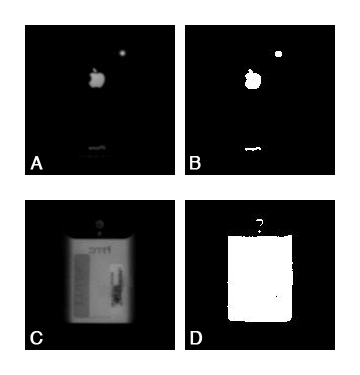
\includegraphics[width=0.5\textwidth]{images/msRaw}
    \caption{Microsoft Surface raw visual input: (A) iPhone 4 (B) iPhone 4 after threshold processing (C) HTC Legend (D) HTC Legend after threshold processing.}
    \label{fig:msRaw}
\end{figure}

The \texttt{TIDEWindow} is an application-specific instance of a \texttt{SurfaceWindow} control provided by the Surface SDK Presentation layer. 
It represents the main application window, and comprises most of the application logic.
It sends screen captures to the \texttt{Tracker} class, that is responsible for processing the images, detecting and tracking the smartphones.
The \texttt{Tracker} keeps track of the devices by using additional tracker classes that are specific to the supported device types.
In the current implementation, the \texttt{IphoneTracker} detects \texttt{Iphone} objects, and the \texttt{LegendTracker} detects \texttt{Legend} objects.
All device types implement the \texttt{IDevice} interface, which provides properties that are used by the main \texttt{Tracker} to keep track of an updated list of current devices.
Upon device apparition, movement or removal, the \texttt{Tracker} raises relevant events, i.e.\ \texttt{DeviceAdded}, \texttt{DeviceUpdated}, \texttt{DeviceRemoved}.
The \texttt{TIDEWindow} listens for such events, and handles them accordingly.

The tracking component provides the application with the means to know when new devices are placed on the table, but also when and where they are moved, and when they are removed entirely.
The initial device detection was used in the evaluated prototype, as a trigger for pairing.

However, the tracking of smartphone devices during the application session was deactivated for the test sessions, for the following reason.
The purpose of tracking devices was to allow the use of the smartphone as a tangible user interface, a remote control for the replicated UI.
This feature was part of the initial requirements, as presented in section~\ref{sec:requirements}, but were left out of the final design, the reasons of which were explained in section~\ref{sec:design}.



%%%%%%%%%%%%%%%%
%% REPLICATION %%
%%%%%%%%%%%%%%%%
\section{Replicated UI}
\label{sec:replicatedui}

The UI replication is based on the VNC protocol \citep{Richardson:1998:vnc}.
The pairing procedure completes with the VNC client on the tabletop connecting to the VNC server running on the smartphone, and receiving the first image of the remote UI.

The VNC client is implemented by the \texttt{VncControl} class, as shown in figure~\ref{fig:surfaceOverview}, that relies on the VncSharp library for sending input and receiving the remote UI.
The \texttt{VncControl} is responsible for displaying the replicated UI, and is contained within a \texttt{DeviceControl} object that provides other UI elements.
When the \texttt{DeviceControl} object detects a contact on the replicated UI, it forwards it to the \texttt{VncControl} object, that relays it further to the smartphone.
The server responds with an updated image of the smartphone's screen, that the \texttt{VncControl} displays on the tabletop.

The VNC server on the smartphones relies currently on third-party applications.
The reason for this was to avoid developing software that would be tied to a certain platform.
It permitted to develop an prototype that can support all types of smartphones, given that they run a VNC server.

However, due to limitations implemented by the manufacturers, installing the VNC applications required rooting the devices.
Rooting a smartphone is a procedure that allows the user to obtain full access rights on the system, though with the implication that the device warranty becomes void.
Thus, it cannot be expected of users that they will perform this procedure, and this approach would be problematic in a real-world scenario.
However, this setup was satisfying for the purpose of the proof-of-concept.

[VNC IS NOT ADAPTED TO THIS SITUATION; IT IS TOO SLOW]

%%%%%%%%%%%%%%
%% SURFACE %%
%%%%%%%%%%%%%%
\section{Surface UI}
\label{sec:surfaceui}

\begin{figure}[htb]
  \centering
    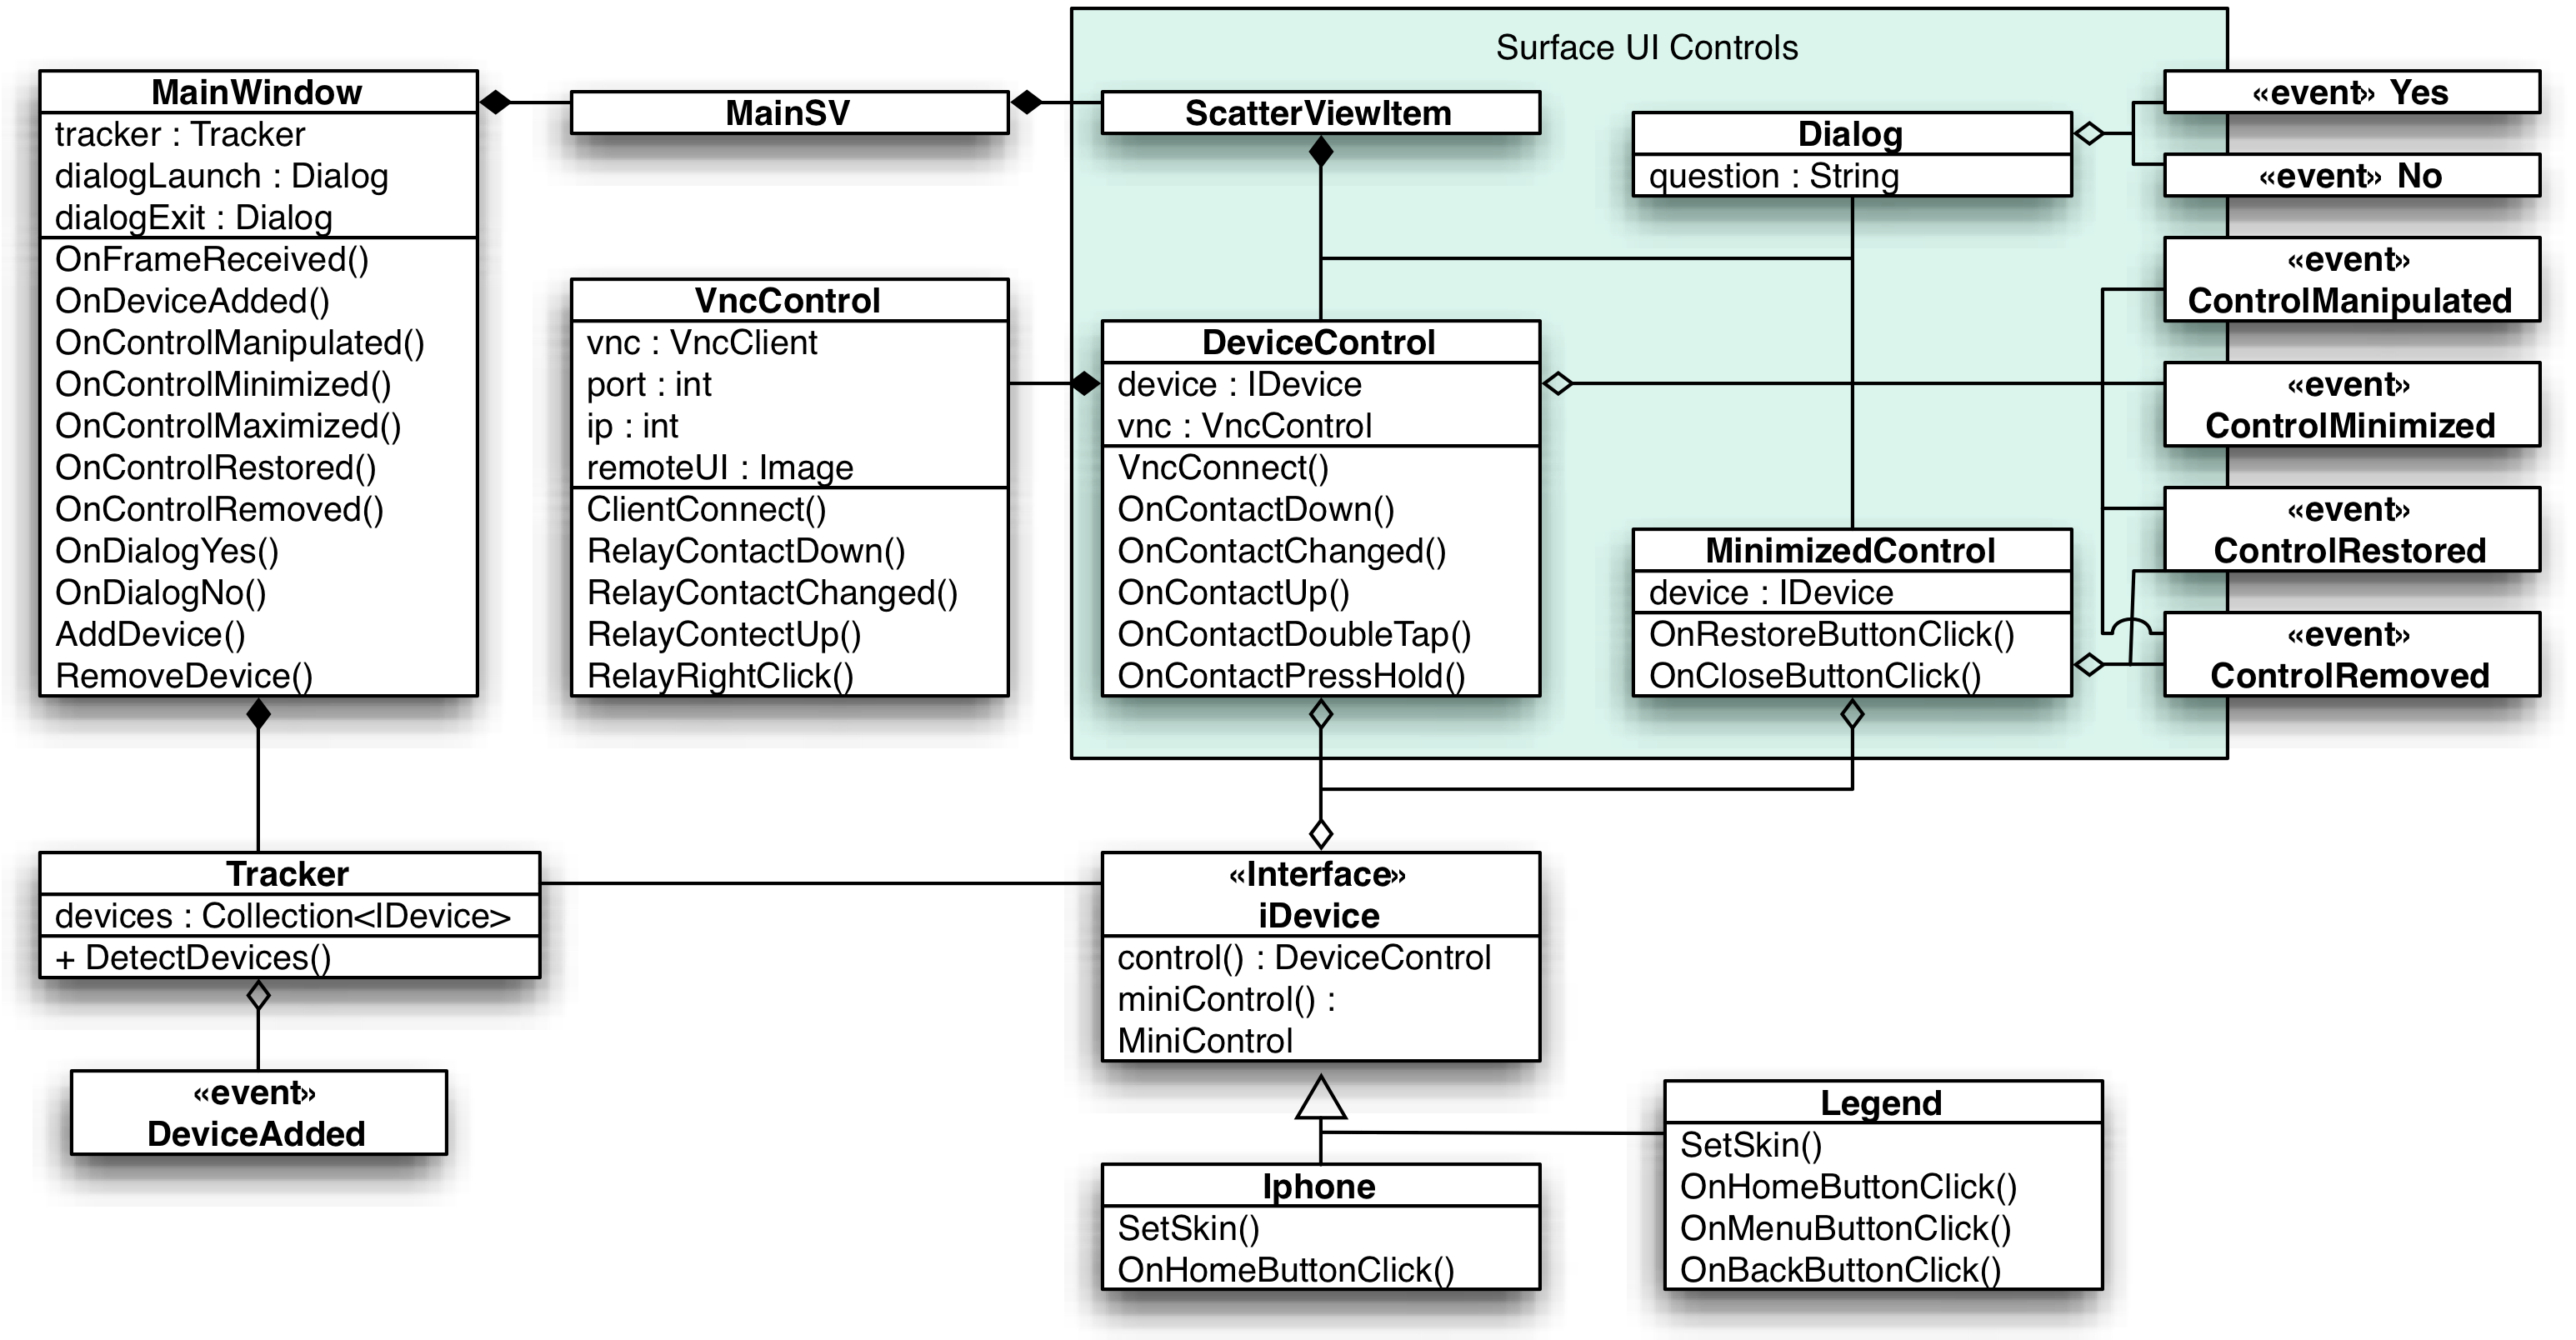
\includegraphics[width=1\textwidth]{images/surfaceDiagram}
    \caption{Surface UI overview.}
    \label{fig:surfaceDiagram}
\end{figure}


\subsection{}

we added MAXIMIZE:
Similarly when enlarged above a certain size, it is maximized to a fullscreen mode. To escape the fullscreen mode, buttons are implemented in the corners of the tabletop.




